\section{Variational equations and the state-transition matrix}\label{app:dxdv}

This appendix collects the equations behind \texttt{Orbit.integrate\_dxdv},
\texttt{Orbit.lyapunov}, and the derivative rule of the \cc\ integrators
of \sectionname~\ref{sec:orbit-paths}. None of it is specific to a
backend; it is implemented in \cc\ and in \numpy.

Write the phase-space coordinates as $\vecw = (\vecx,\vecv)$ in
rectangular Galactocentric coordinates, in which \galpy's \cc\
integrators work, and the equations of motion as $\dot{\vecw} =
\vec{f}(\vecw,t)$ with $\dot{\vecx} = \vecv$ and $\dot{\vecv} =
\vec{a}(\vecx,\vecv,t)$. A small deviation $\delta\vecw$ from an orbit
evolves according to the linearized equations
\begin{equation}\label{eq:variational}
  \frac{\dd\,\delta\vecw}{\dd t} = \vec{J}(t)\,\delta\vecw\,,\qquad
  \vec{J} = \begin{pmatrix} \vec{0} & \vec{I} \\
    \partial\vec{a}/\partial\vecx & \partial\vec{a}/\partial\vecv\end{pmatrix}\,,
\end{equation}
evaluated along the orbit. For a conservative force,
$\partial\vec{a}/\partial\vecv = \vec{0}$ and $\vec{K} \equiv
\partial\vec{a}/\partial\vecx = -\nabla\nabla\Phi$ is the symmetric
Hessian of the potential. \galpy's potentials provide their second
derivatives in cylindrical coordinates, and $\vec{K}$ is assembled from
them: with $\cos\phi = x/R$ and $\sin\phi = y/R$, the in-plane block is
the one of the planar variational equations that \galpy\ has had since
2011, built from $\partial^2\Phi/\partial R^2$,
$\partial^2\Phi/\partial\phi^2$, and $\partial^2\Phi/\partial R\partial\phi$,
and the vertical couplings are
\begin{align}
  K_{xz} &= -\cos\phi\,\frac{\partial^2\Phi}{\partial R\partial z}
            +\frac{\sin\phi}{R}\,\frac{\partial^2\Phi}{\partial z\partial\phi}\,,\nonumber\\
  K_{yz} &= -\sin\phi\,\frac{\partial^2\Phi}{\partial R\partial z}
            -\frac{\cos\phi}{R}\,\frac{\partial^2\Phi}{\partial z\partial\phi}\,,\\
  K_{zz} &= -\frac{\partial^2\Phi}{\partial z^2}\,.\nonumber
\end{align}
The mixed derivatives $\partial^2\Phi/\partial R\partial z$ and
$\partial^2\Phi/\partial z\partial\phi$ were added to the \cc\ interface
of every potential for this purpose, and the symmetry of $\vec{K}$ is
checked by the test suite. For a dissipative force
$\vec{F}(\vecx,\vecv)$, such as dynamical friction, the lower-right
block $\partial\vec{F}/\partial\vecv$ is non-zero and the lower-left
block is not symmetric; both are implemented for \galpy's
dynamical-friction forces.

The state-transition matrix $\vec{M}(t) = \partial\vecw(t)/\partial\vecw(0)$
is the solution of \eqnname~(\ref{eq:variational}) for six independent
deviation vectors, $\dot{\vec{M}} = \vec{J}\vec{M}$ with
$\vec{M}(0) = \vec{I}$. The Runge--Kutta integrators integrate the orbit
and all six columns as one 42-component state, such that the deviations
see the same steps as the orbit; the symplectic integrators apply to the
deviations the drift ($\delta\vecx \leftarrow \delta\vecx +
h\,\delta\vecv$) and kick ($\delta\vecv \leftarrow \delta\vecv +
h\,\vec{K}\,\delta\vecx$) sub-steps with the same coefficients as the
orbit, which is the tangent map of the integrator and is itself
symplectic. For a conservative force, $\vec{M}$ is symplectic,
$\vec{M}^T\boldsymbol{\Omega}\vec{M} = \boldsymbol{\Omega}$ with
$\boldsymbol{\Omega}$ the standard symplectic form, and in particular
$\det\vec{M} = 1$, which is Liouville's theorem; for a dissipative force,
$\det\vec{M}(t) = \exp\int_0^t \mathrm{tr}\,(\partial\vec{F}/\partial\vecv)\,\dd t'$,
which measures the contraction of phase-space volume. These identities
are necessary but not sufficient checks---a sign error in one block of
$\vec{K}$ can leave the determinant equal to one---and the test that
settles the correctness of $\vec{M}$ is the comparison of its columns
with finite differences of independently integrated orbits, in which the
finite-difference error follows its characteristic V shape with step
size and the variational result sits at the bottom of the V.
\figurename~\ref{fig:variational} shows these checks for a Milky-Way
orbit: the Liouville and symplecticity defects stay below $10^{-6}$ over
a hundred time units, and the state-transition matrix agrees with the
best central difference at the finite-difference floor of $10^{-8}$.

\begin{figure}[t!]
  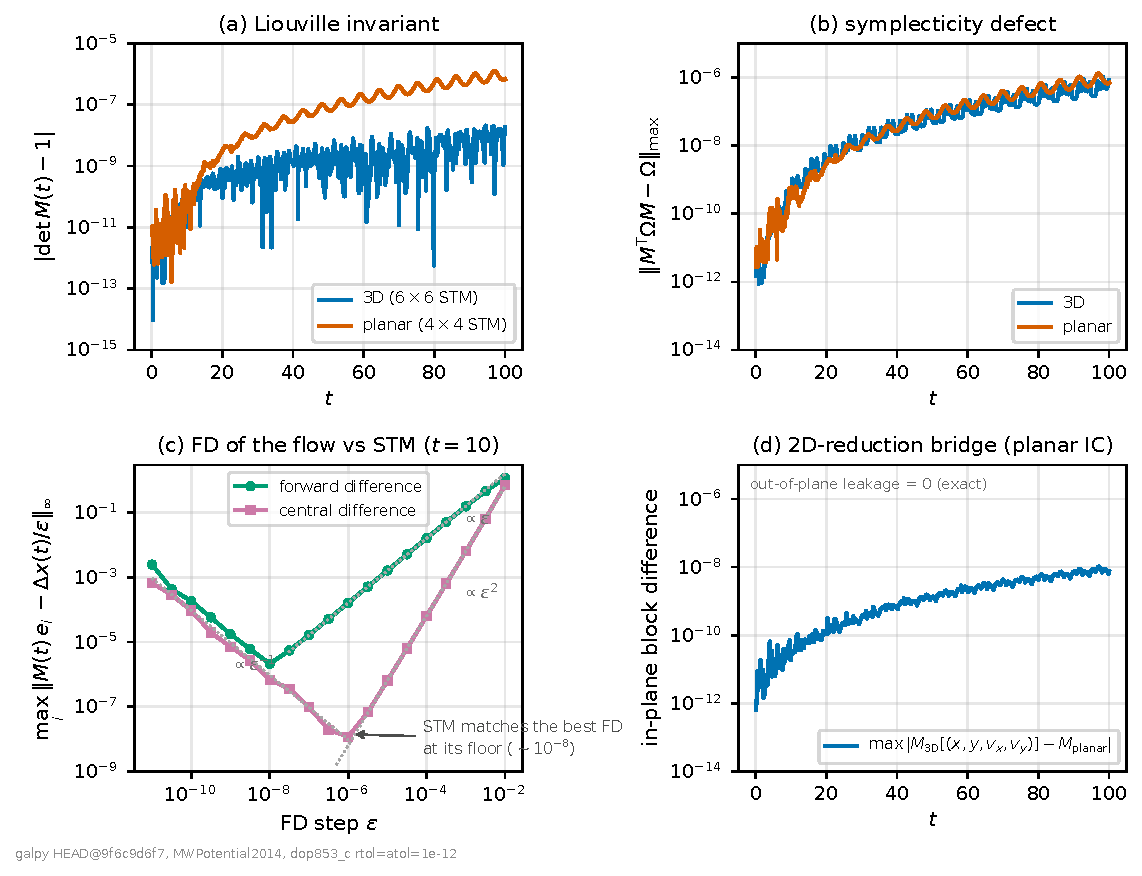
\includegraphics[width=0.48\textwidth,clip=]{../figures/g9_variational_validity/g9_variational_validity.pdf}
  \caption{Checks of the \cc\ variational equations for an orbit in
    \texttt{MWPotential2014}, integrated with \texttt{dop853\_c} at
    tolerances of $10^{-12}$. (a) The Liouville defect $|\det\vec{M}-1|$
    and (b) the symplecticity defect for the three-dimensional and the
    planar state-transition matrix. (c) The difference between the
    columns of $\vec{M}$ at $t=10$ and forward and central finite
    differences of independently integrated orbits as a function of the
    finite-difference step; the variational result agrees with the best
    central difference at its floor. (d) The in-plane block of the
    three-dimensional matrix for a planar initial condition agrees with
    the planar matrix, with no leakage out of the plane.}\label{fig:variational}
\end{figure}

The derivative rule of \sectionname~\ref{sec:orbit-paths} follows from
the chain rule: for a scalar function $L$ of the orbit sampled at times
$t_k$, $\partial L/\partial\vecw(0) = \sum_k \vec{M}(t_k)^T\,
\partial L/\partial\vecw(t_k)$, which is a single matrix--vector product
per output time once $\vec{M}$ is known. Lyapunov exponents are
computed by integrating a deviation vector with
\eqnname~(\ref{eq:variational}), renormalizing it to unit length every
fixed number of steps, and accumulating the logarithms of the
normalization factors \citep{Benettin1980a,Benettin1980b}; the spectrum follows by
orthonormalizing a set of deviation vectors in the same way.
